%%%%%%%%%%%%%%%%%%%%%%%%%%%%%%%%%%%%%%%%%
% Short Sectioned Assignment
% LaTeX Template
% Version 1.0 (5/5/12)
%
% This template has been downloaded from:
% http://www.LaTeXTemplates.com
%
% Original author:
% Frits Wenneker (http://www.howtotex.com)
%
% License:
% CC BY-NC-SA 3.0 (http://creativecommons.org/licenses/by-nc-sa/3.0/)
%
%%%%%%%%%%%%%%%%%%%%%%%%%%%%%%%%%%%%%%%%%

%----------------------------------------------------------------------------------------
%	PACKAGES AND OTHER DOCUMENT CONFIGURATIONS
%----------------------------------------------------------------------------------------

\documentclass[paper=a4, fontsize=11pt]{scrartcl} % A4 paper and 11pt font size

\usepackage{tikz}
\usepackage[T1]{fontenc} % Use 8-bit encoding that has 256 glyphs
\usepackage{fourier} % Use the Adobe Utopia font for the document - comment this line to return to the LaTeX default
\usepackage[american]{babel} % English language/hyphenation
\usepackage{amsmath,amsfonts,amsthm} % Math packages

\usepackage{csquotes}
\usepackage[style=apa,sortcites=true,sorting=nyt,backend=biber]{biblatex} %bibliography package
\DeclareLanguageMapping{american}{american-apa}
\nocite{*}

\usepackage{sectsty} % Allows customizing section commands
\allsectionsfont{\centering \normalfont\scshape} % Make all sections centered, the default font and small caps

\usepackage{fancyhdr} % Custom headers and footers
\usepackage{outlines}
\usepackage{enumitem}

\pagestyle{fancyplain} % Makes all pages in the document conform to the custom headers and footers
\fancyhead{} % No page header - if you want one, create it in the same way as the footers below
\fancyfoot[L]{} % Empty left footer
\fancyfoot[C]{} % Empty center footer
\fancyfoot[R]{\thepage} % Page numbering for right footer
\renewcommand{\headrulewidth}{0pt} % Remove header underlines
\renewcommand{\footrulewidth}{0pt} % Remove footer underlines
\setlength{\headheight}{13.6pt} % Customize the height of the header

\numberwithin{equation}{section} % Number equations within sections (i.e. 1.1, 1.2, 2.1, 2.2 instead of 1, 2, 3, 4)
\numberwithin{figure}{section} % Number figures within sections (i.e. 1.1, 1.2, 2.1, 2.2 instead of 1, 2, 3, 4)
\numberwithin{table}{section} % Number tables within sections (i.e. 1.1, 1.2, 2.1, 2.2 instead of 1, 2, 3, 4)

\setlength\parindent{0pt} % Removes all indentation from paragraphs - comment this line for an assignment with lots of text

\bibliography{biblio}
%----------------------------------------------------------------------------------------
%	TITLE SECTION
%----------------------------------------------------------------------------------------

\newcommand{\horrule}[1]{\rule{\linewidth}{#1}} % Create horizontal rule command with 1 argument of height

\title{	
\normalfont \normalsize 
\textsc{Math 460} \\ [25pt] % Your university, school and/or department name(s)
\horrule{0.5pt} \\[0.4cm] % Thin top horizontal rule
\huge Golay Codes\\ % The assignment title
\horrule{2pt} \\[0.5cm] % Thick bottom horizontal rule
}

\author{Dean Bisogno} % Your name

\date{\normalsize\today} % Today's date or a custom date
\newtheorem{defn}{Definition}
\newtheorem{thm}{Theorem}
\newtheorem{lma}{Lemma}
\setenumerate[1]{label=\Roman*.}
\setenumerate[2]{label=\Alph*.}
\setenumerate[3]{label=\roman*.}
\setenumerate[4]{label=\alph*.}

\begin{document}
\maketitle % Print the title

\section{History and Construction}

The binary Golay code has been pivotal in understanding the 
\begin{outline}[enumerate]
   \1 Constructions of the perfect Golay $[23,12,7]$ code $\mathcal{G}_{23}$ and extended (not perfect) $[24,12,8]$ Golay $[24,12,8]$ code $\mathcal{G}_{24}$.
       \2 As the $S(5,8,24)$ Steiner System [\cite{griess}]
         \3 Steiner Systems
           \begin{defn}{Steiner system}

            A Steiner system with parameters (a,b,c) is a family $S$ of subsets of some set $\Omega$ of c elements such that (i) $A \in S$ implies that $|A| = b$; (ii) for any a-set \textit{F} in $\Omega$, there is a unique $A \in S$ such that $\textit{F} \subseteq A$.
           \end{defn}
         \3 Fano plane as example of S(2,3,7). Seven lines partition the seven points, where each line contains exactly three points, and each pair of points uniquely designates a line.
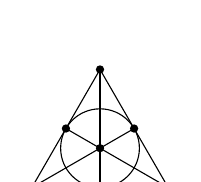
\begin{tikzpicture}

   \draw (0,0) circle (0.5);
   \draw (90:1) -- (-30:1)--(210:1)--cycle;

   \draw (90:1)--(0,0);
   \draw (210:1)--(0,0);
   \draw (-30:1)--(0,0);

   \draw (30:0.5)--(0,0);
   \draw (150:0.5)--(0,0);
   \draw (270:0.5)--(0,0);

   \fill (-0.866,-0.5) circle (1.5pt);
   \fill (0.866,-0.5) circle (1.5pt);
   \fill (0,-0.5) circle (1.5pt);
   \fill (0,1) circle (1.5pt);
   \fill (0,0) circle (1.5pt);
   \fill (0.433,0.25) circle (1.5pt);
   \fill (-0.433,0.25) circle (1.5pt);

\end{tikzpicture}


      \2 Generator Matrix as [I:A] where A is the adjacency matrix of the icosahedron.
      \2 Perfect $\mathcal{G}_{23}$ created by removing the parity digit.
\end{outline}

\section{Important Properties}
\begin{outline}[enumerate]
  \1 Important properties of the Golay Codes
       \2 Octads, dodecads, and sextets
         \begin{defn}{Octads, dodecad, and sextets}

           For $S(5,8,24)$ we call elements of $S$ octads, a dodecad is a 12-set, a sextet is a 4-set (the sextets partition the space into six set).
         \end{defn}
      \2 Minimum weight of $\mathcal{G}_{24}$ is 8, other codeword weights are 12, 16, and 24. We can detect 7 errors and correct $3 = \lfloor \frac{8-1}{2} \rfloor$. This is where we see that $\mathcal{G}_{24}$ is not perfect because spheres of radius 4 centered at codewords intersect while spheres of radius 3 do not fill the space. 
      \2 Self-duality [\cite{ivanov}]
         \begin{defn}{dual code}

          For a code $\mathcal{C}$, the dual code $\mathcal{C}^*$ is the orthogonal complement of $\mathcal{C}$ with respect to the parity form. ie. $\mathcal{C}^{*} = \{A | A \in 2^X, |A \cap B|$ is even for all $B \in \mathcal{C} \}.$
         \end{defn}
         \begin{defn}{totally singular}

          We call a code $\mathcal{C}$ totally singular if $\mathcal{C} \subseteq \mathcal{C}^*$.
         \end{defn}
         \begin{lma}
          A code $\mathcal{C}$ of length $X$ is self-dual if it is totally singular with respect to the parity form and $dim(\mathcal{C}) = |X|/2$.
         \end{lma}
\end{outline}
\section{The Automorphism Group $M_{24}$}
\begin{outline}[enumerate]
   \1 Automorphism Group of $\mathcal{G}_{24}$.       
       \2 The hexacode and Miracle Octad Generator (MOG) are valuable tools when working with $\mathcal{G}_{24}$ because it gives us a method to quickly check whether a message is a valid codeword. It also becomes useful when investigating maximal subgroups of $Aut(\mathcal{G}_{24})$ [\cite{conway}].

       \begin{defn}{Hexacode}

        Consider $\mathbb{F}_4 = \{0,1,\alpha,\bar{\alpha}\}$ with the usual relations.
        Then hexacode $\mathcal{C}_6$ has a word $W(\phi) = ab|cd|ef$ for each quadratic function $\phi(x) = ax^2 + bx + c$ defined over $\mathbb{F}_4$. Where $c=\phi(0)$, $d=\phi(1)$, $e=\phi(\alpha)$, $f=\phi(\bar{\alpha})$.

        We can also consider $\mathcal{C}_6$ to be generated by 
        $$\alpha\bar{\alpha}|\alpha\bar{\alpha}|\alpha\bar{\alpha}$$
        $$\alpha\bar{\alpha}|\bar{\alpha}\alpha|\bar{\alpha}\alpha$$
        $$\bar{\alpha}\alpha|\alpha\bar{\alpha}|\bar{\alpha}\alpha$$
        $$\bar{\alpha}\alpha|\bar{\alpha}\alpha|\alpha\bar{\alpha}.$$
       \end{defn}
       \2 k-fold transitivity
          \begin{defn}
             Let G be a group acting on a set $\Omega$, and $k \leq |\Omega|$. We say that G is k-fold transitive on $\Omega$ if, given any two ordered k-tuples $(x_1, \ldots, x_k)$ and $(y_1, \ldots, y_k)$, there is an element $g \in G$ such that $x_ig = y_i$ for all $i \in {1, \ldots, k}$. If such a $g \in G$ is unique, then we call G sharply k-fold transitive on $\Omega$.
          \end{defn}
       \2 We will find that $Aut(\mathcal{G}_{24}) = M_{24}$ where $M_{24}$ is a 5-fold transitive, simple permutation group on 24 points. We can also show that $|M_{24}| = 2^{10} \times 3^3 \times 5 \times 7 \times 23 = 244,823,040$.

\end{outline}
\clearpage
\printbibliography
%----------------------------------------------------------------------------------------

\end{document}